\documentclass[../the.tex]{subfiles}


\begin{document}

Trong chương này sẽ trình bày phần phân tích kết quả của mô hình được đề xuất trong Mục \ref{sec:result}. Các nghiên cứu liên quan và các vấn đề trong việc phát hiện gãy xương được thảo luận trong Mục \ref{sec:result_related}.

\section{Phân tích kết quả của mô hình}
\label{sec:result}

\subsection{Kết quả phát hiện gãy xương}

{\fontsize{13}{12} \selectfont
Trong các Bảng \ref{tab:binary},\ref{tab:image},\ref{tab:frac} trình bày các kết quả tương ứng cho các tiêu chuẩn đánh giá mô hình dựa trên nhị phân, dựa trên hình ảnh và dựa trên đứt gãy (kết quả tốt nhất được nhấn mạnh). Các bảng này cũng chứa các giá trị của các ngưỡng được sử dụng, cho mỗi mô hình. Các ngưỡng được đặt theo kết quả đạt được tốt nhất của họ trên tập dữ liệu xác thực, như đã mô tả trong Mục \ref{sec:dataset}.

Trong cả ba lần đánh giá, mô hình YOLO 512 mỏ neo đạt kết quả tốt nhất trong khi mô hình U-Net liên tục kém nhất. Precision là chỉ số duy nhất mà mô hình YOLO 512 mỏ neo không hoạt động tốt nhất trong cả ba lần đánh giá. Cụ thể, để đánh giá dựa trên hình ảnh (Bảng \ref{tab:image}, và Hình \ref{fig:chart_1}) và dựa trên vết gãy (Bảng \ref{tab:frac} và Hình \ref{fig:chart_2}), mô hình YOLO 608 mỏ neo đã đạt được điểm chính xác tốt nhất. Đối với đánh giá nhị phân (Bảng \ref{tab:binary} và Hình \ref{fig:chart_3}), mô hình YOLO 512 mỏ neo đạt được độ chính xác tốt nhất.


Trong Hình \ref{fig:predict_1}, \ref{fig:predict_2}, và \ref{fig:predict_3} so sánh các vị trí gãy xương được phát hiện bởi mô hình và các vị trí gãy xyơng thực sự (được đánh dấu bởi các bác sĩ). Các hộp màu xanh là những vị trí được các bác sĩ kiểm tra và đánh dấu trong khi màu đỏ là những vị trí được xác định bởi mô hình.
}

% Bang 1
\begin{table}[ht!]
\centering
\caption{Đánh giá nhị phân của các mô hình trong tập thử nghiệm \# 1 (in đậm thể hiện giá trị vượt trội).}
\begin{tabular}{|c|c|c|c|c|}
\hline
\textbf{Model}
& \textbf{Precision}
& \textbf{Recall}  
& \textbf{F$_{1}$} 
& \textbf{Accuracy} 
\\ \hline 
YOLO 512           & 0,94658       & 0,94667   & 0,94661    & 0,94667     \\  \hline
YOLO 512 mỏ neo   & \textbf{0,94969}       & \textbf{0,94974}   & \textbf{0,94971}    & \textbf{0,94974}     \\  \hline
YOLO 608           & 0,94311       & 0,94205   & 0,94233    & 0,94205     \\  \hline
YOLO 608 mỏ neo   & 0,94264       & 0,94103   & 0,94139    & 0,94103     \\  \hline
U-Net              & 0,92268       & 0,92154   & 0,92189    & 0,92154     \\  \hline

\end{tabular}
\label{tab:binary}

\end{table}

% Bang 2

\begin{table}[h!]
\centering
\caption{Đánh giá dựa trên hình ảnh của các mô hình trong tập thử nghiệm \# 1 (in đậm thể hiện giá trị vượt trội).}
\begin{tabular}{|c|c|c|c|c|}
\hline
\textbf{Model}
& \textbf{Precision}
& \textbf{Recall}  
& \textbf{F$_{1}$} 
& \textbf{Accuracy} 
\\ \hline 
YOLO 512           & 0,86455       & 0,85385   & 0,85556    & 0,85385     \\  \hline
YOLO 512 mỏ neo   & 0,86470       & \textbf{0,85846}   & \textbf{0,85973}    & \textbf{0,85846}     \\  \hline
YOLO 608           & 0,86063       & 0,84923   & 0,85103    & 0,84923     \\  \hline
YOLO 608 mỏ neo   & \textbf{0,86570}       & 0,84821   & 0,85051    & 0,84821     \\  \hline
U-Net              & 0,74644       & 0,72359   & 0,72516    & 0,72359     \\  \hline


\end{tabular}
\label{tab:image}
\end{table}


% Bang 3

\begin{table}[h!]
\centering
\caption{Đánh giá dựa trên gãy xương của các mô hình trong tập thử nghiệm \# 1 (in đậm thể hiện giá trị vượt trội).}
\begin{tabular}{|c|c|c|c|c|}
\hline
\textbf{Model}
& \textbf{Precision}
& \textbf{Recall}  
& \textbf{F$_{1}$} 
& \textbf{Accuracy} 
\\ \hline 
YOLO 512           & 0,89997       & 0,89144   & 0,89327    & 0,89144     \\  \hline
YOLO 512 mỏ neo   & 0,90369       & \textbf{0,89871}   & \textbf{0,89997}    & \textbf{0,89871}     \\  \hline
YOLO 608           & 0,89718       & 0,88701   & 0,88907    & 0,88701     \\  \hline
YOLO 608 mỏ neo   & \textbf{0,90502}       & 0,89387   & 0,89592    & 0,89387     \\  \hline
U-Net              & 0,84805       & 0,82889   & 0,83292    & 0,82889     \\  \hline

\end{tabular}
\label{tab:frac}
\end{table}

\begin{figure}[H]
\centering
	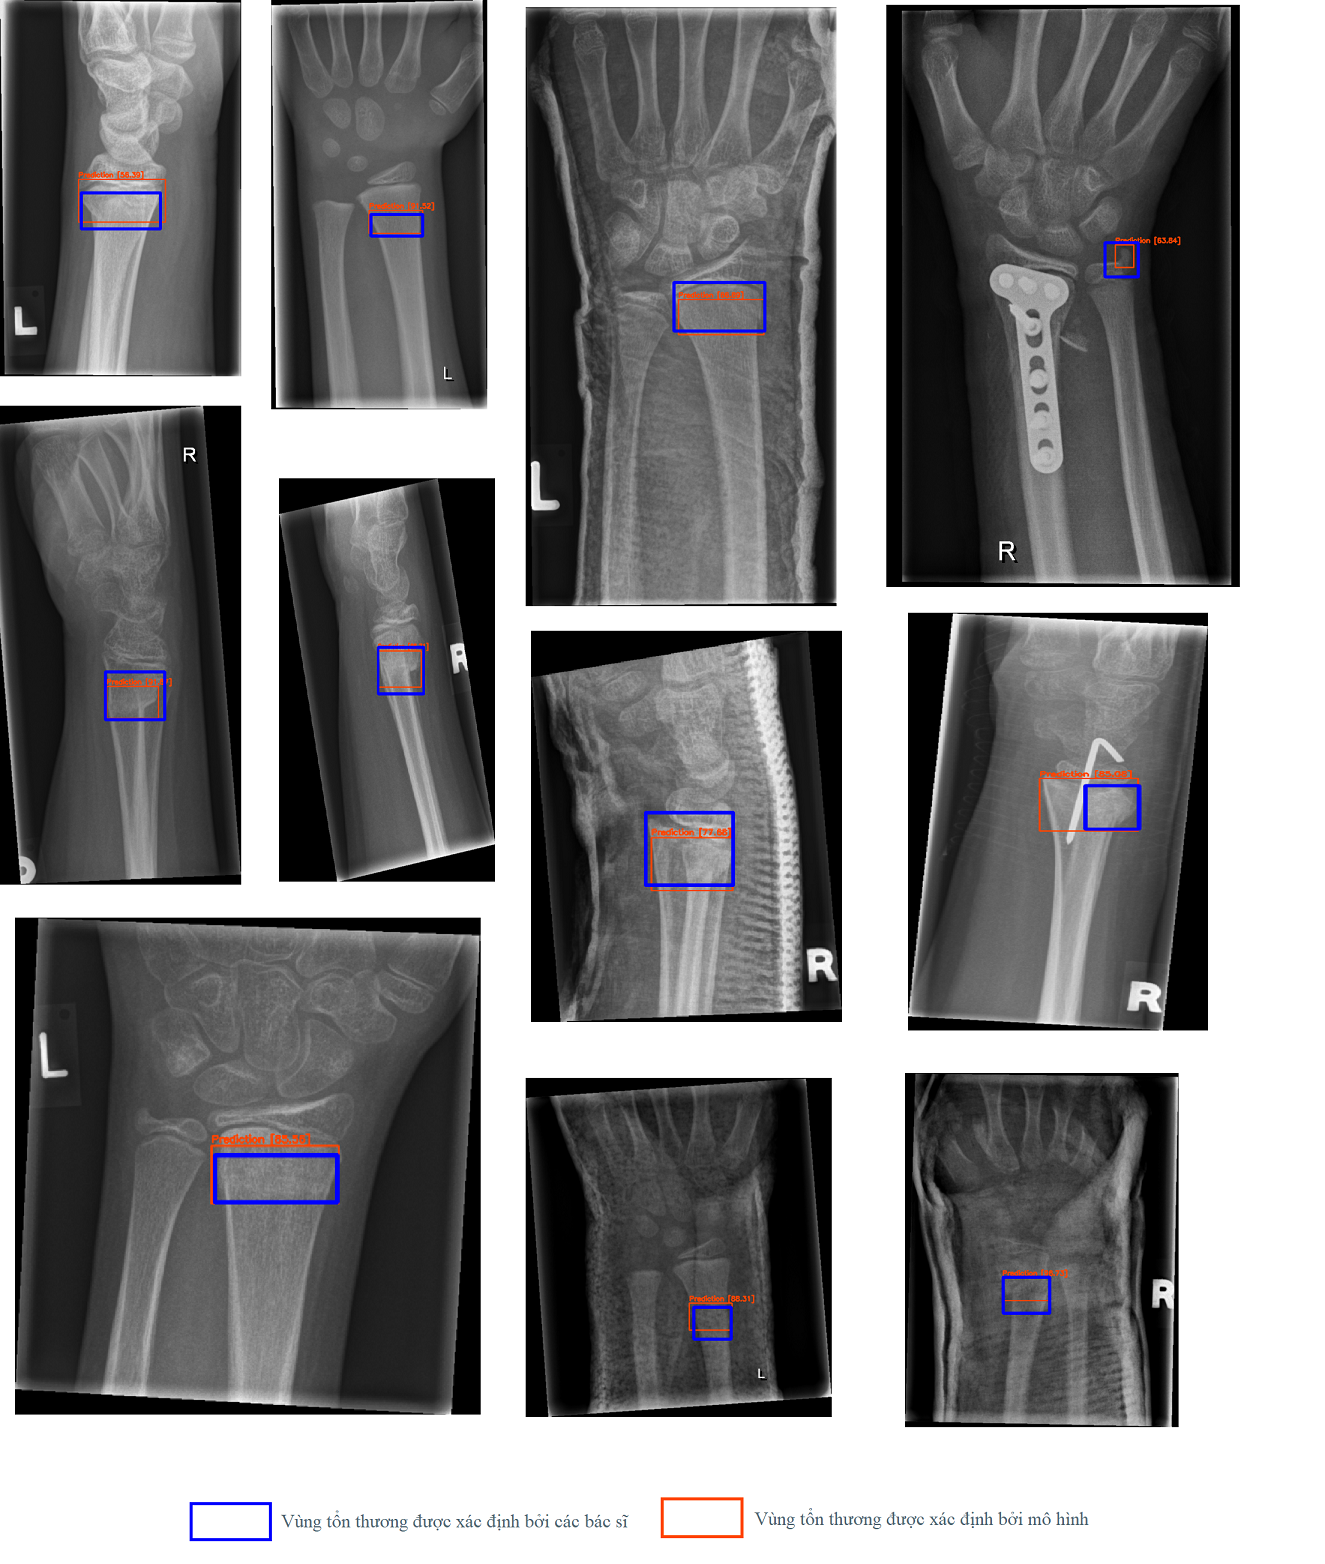
\includegraphics[width=0.95\textwidth]{images/predict_1.png}
	\caption{Kết quả dự đoán vị trí gãy xương của mô hình so với vị trí gãy thực sự - Trường hợp ảnh có một vết gãy. Hộp màu xanh là vị trí gãy thực sự, màu đỏ là vị trí gãy phát hiện bởi mô hình.}
	\label{fig:predict_1}
\end{figure}

\begin{figure}[H]
\centering
	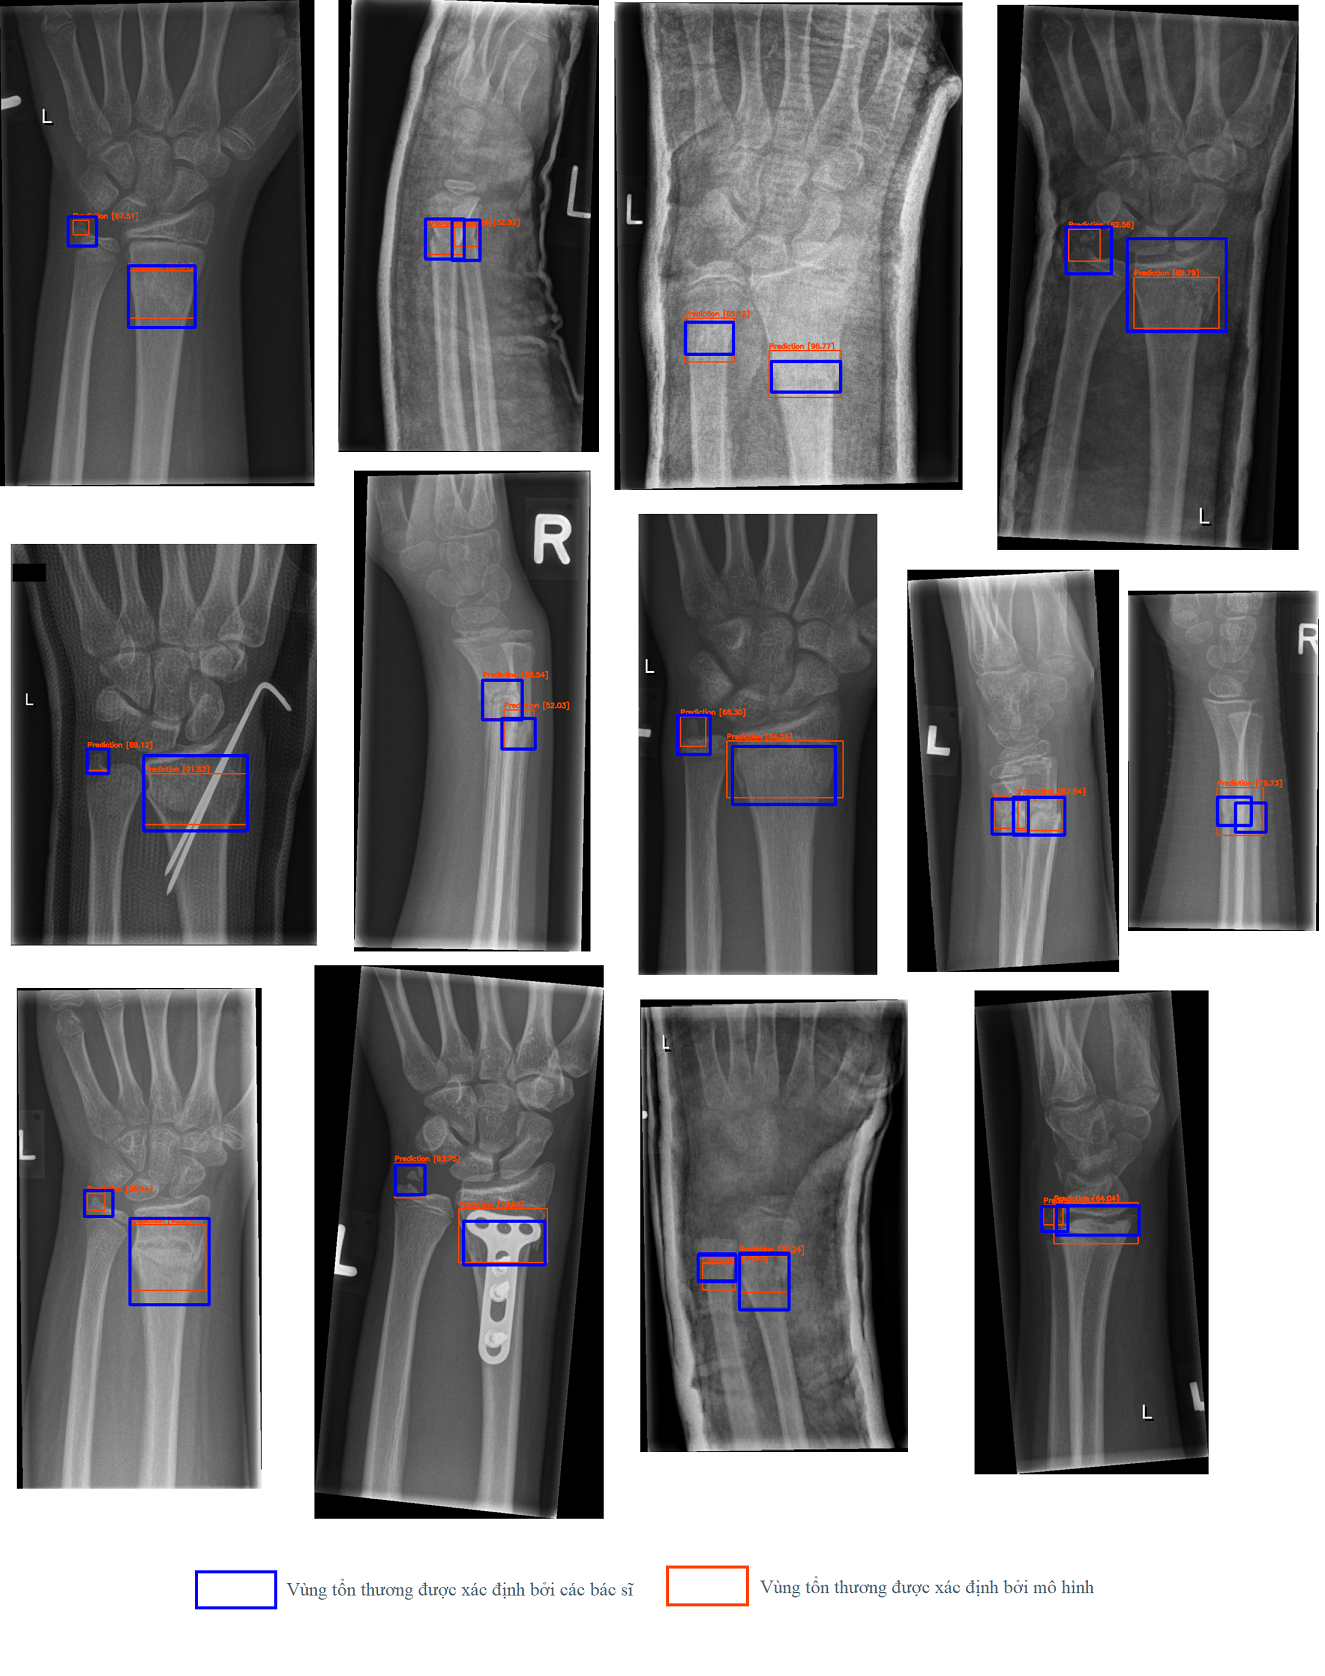
\includegraphics[width=1\textwidth]{images/predict_2.png}
	\caption{Kết quả dự đoán vị trí gãy xương của mô hình so với vị trí gãy thực sự - Trường hợp ảnh có hai vết gãy. Hộp màu xanh là vị trí gãy thực sự, màu đỏ là vị trí gãy phát hiện bởi mô hình.}
	\label{fig:predict_2}
\end{figure}

\begin{figure}[H]
\centering
	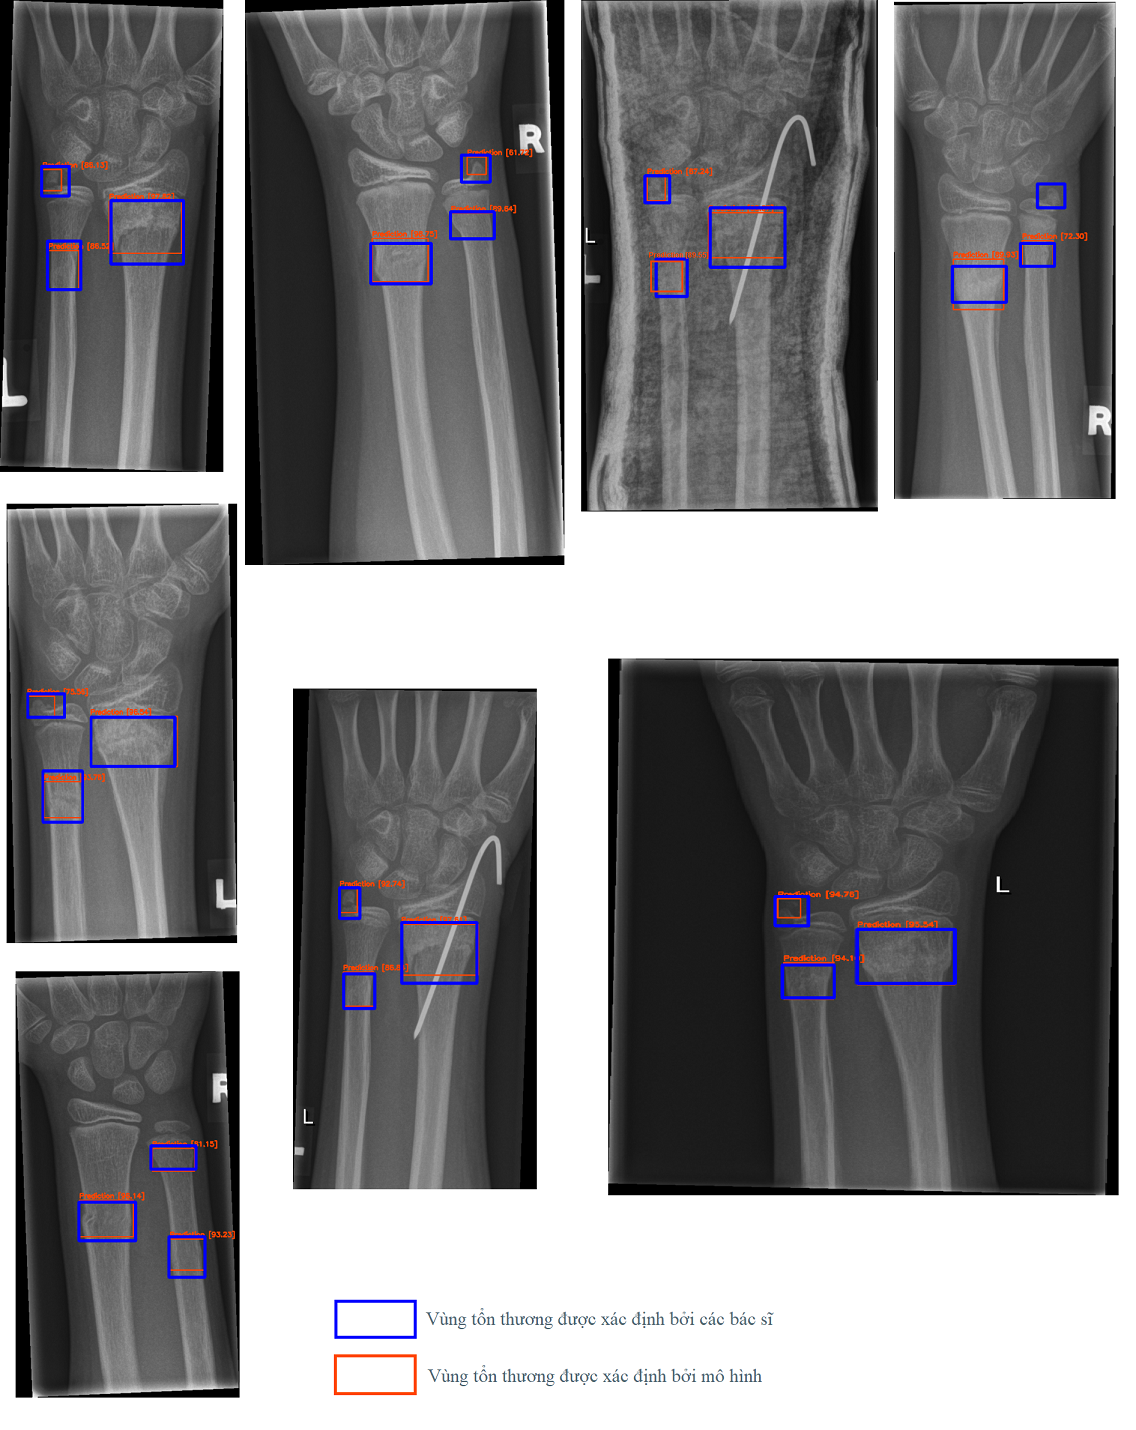
\includegraphics[width=1\textwidth]{images/predict_3.png}
	\caption{Kết quả dự đoán vị trí gãy xương của mô hình so với vị trí gãy thực sự - Trường hợp ảnh có ba vết gãy. Hộp màu xanh là vị trí gãy thực sự, màu đỏ là vị trí gãy phát hiện bởi mô hình.}
	\label{fig:predict_3}
\end{figure}

\begin{figure}[ht!]
\centering
	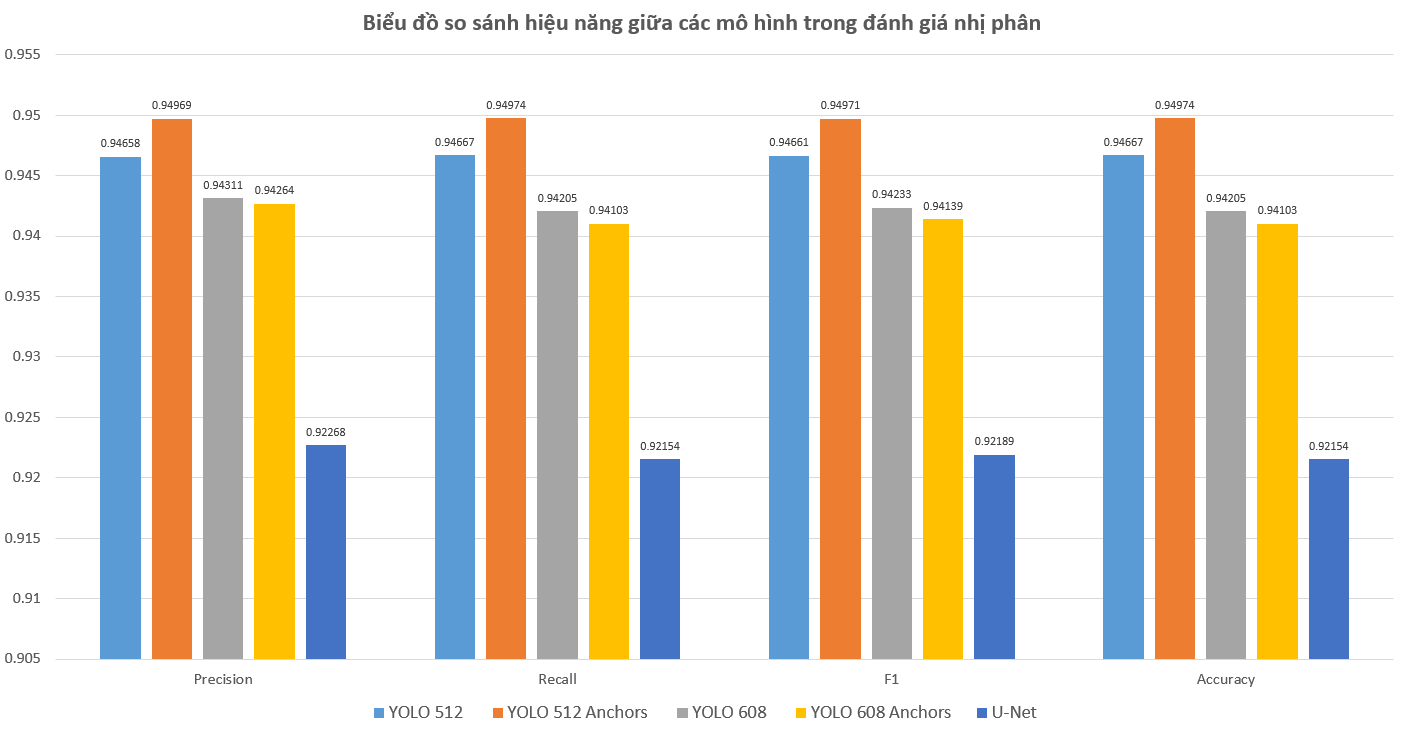
\includegraphics[width=1\textwidth]{images/chart_1.PNG}
	\caption{Biểu đồ so sánh hiệu năng giữa các mô hình trên đánh giá nhị phân.}
	\label{fig:chart_1}
\end{figure}

\begin{figure}[ht!]
\centering
	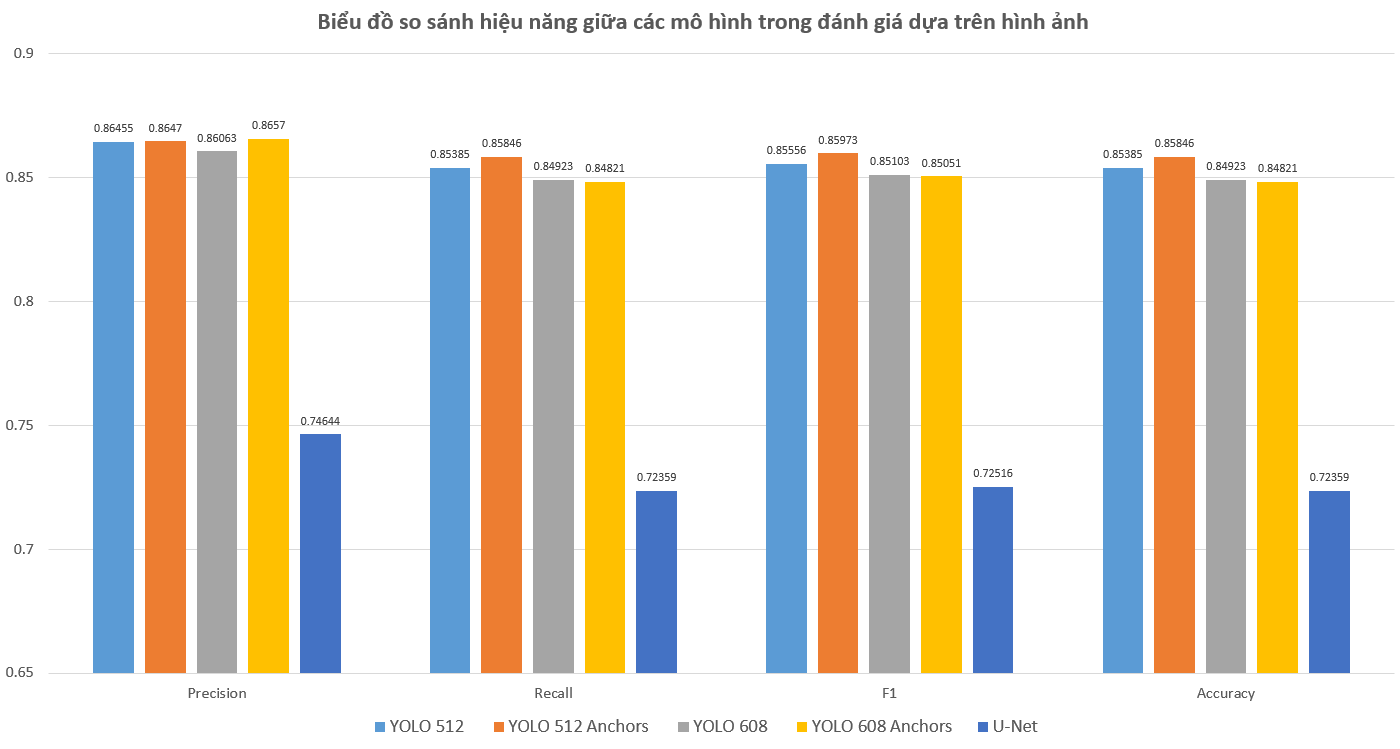
\includegraphics[width=1\textwidth]{images/chart_2.PNG}
	\caption{Biểu đồ so sánh hiệu năng giữa các mô hình trên đánh giá dựa trên hình ảnh.}
	\label{fig:chart_2}
\end{figure}

\begin{figure}[ht!]
\centering
	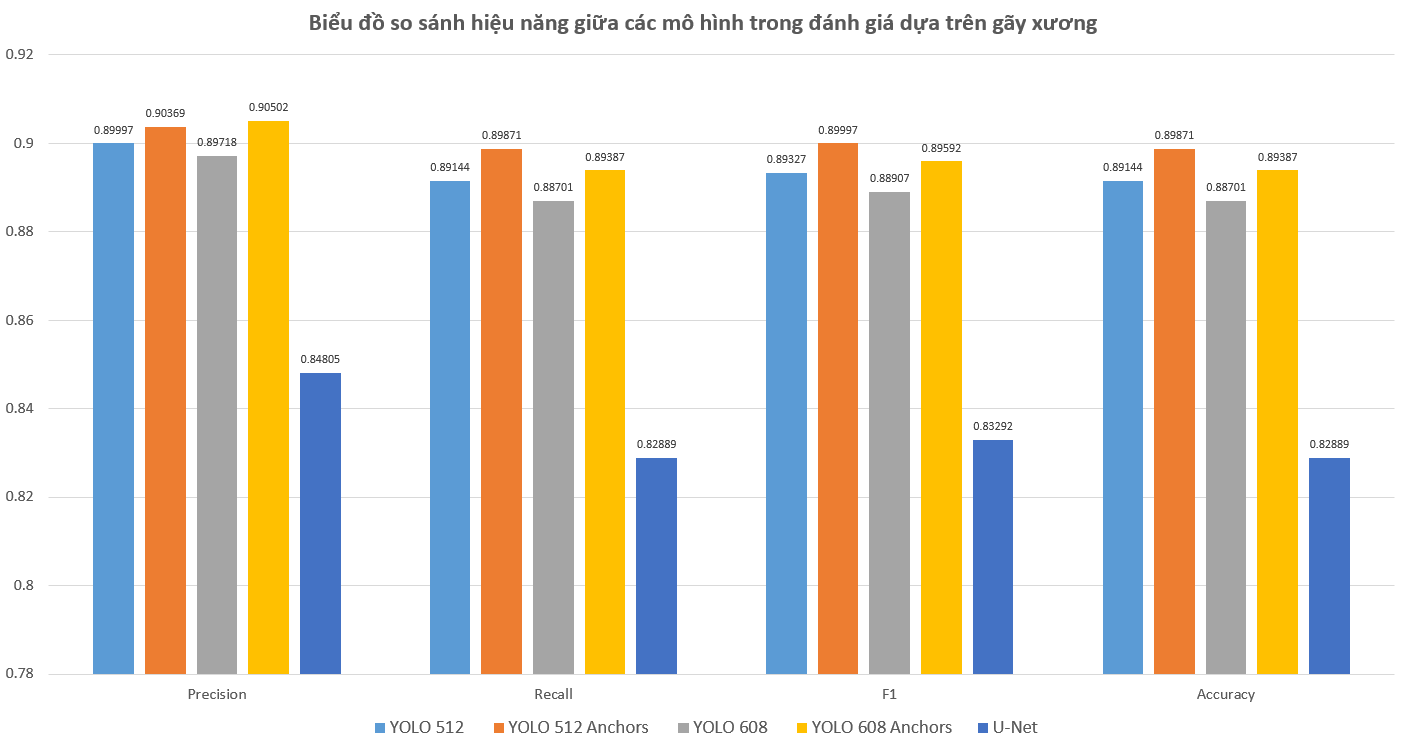
\includegraphics[width=1\textwidth]{images/chart_3.PNG}
	\caption{Biểu đồ so sánh hiệu năng giữa các mô hình trên đánh giá dựa trêngãy xương.}
	\label{fig:chart_3}
\end{figure}

% \begin{figure}[ht!]
% \centering
% 	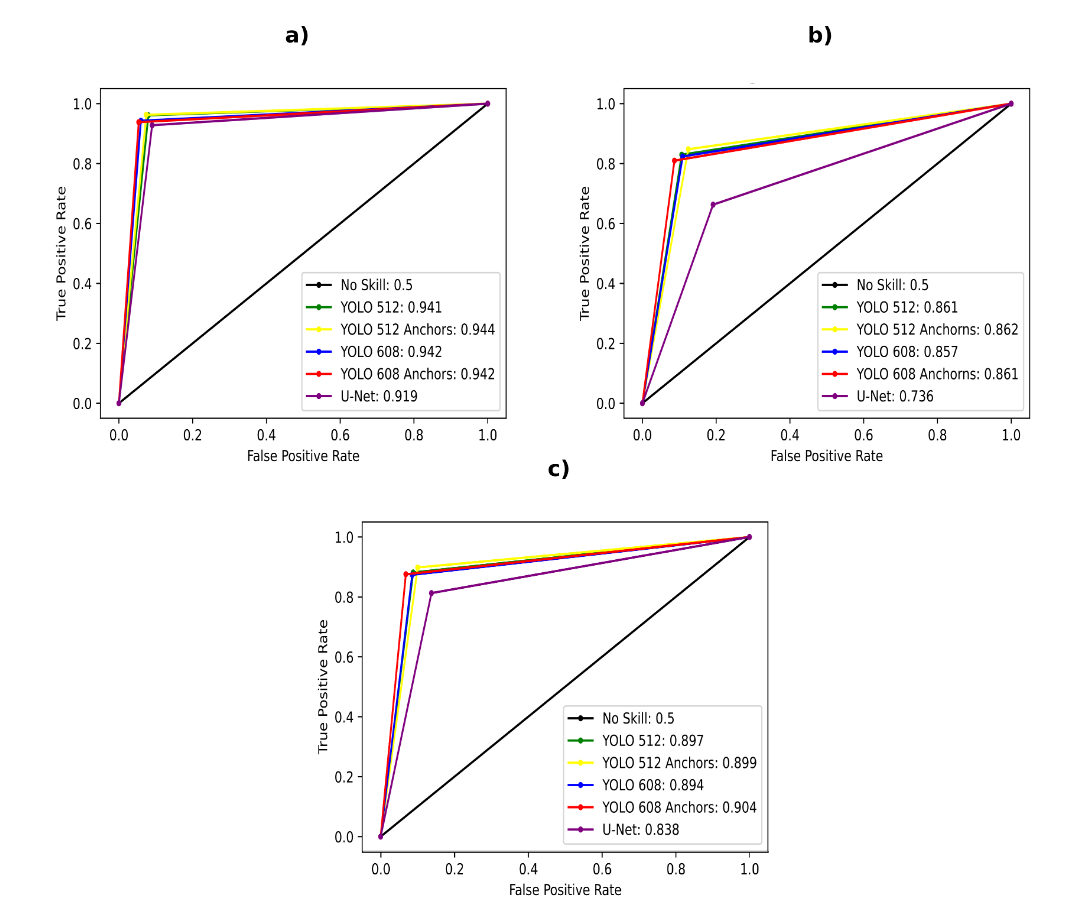
\includegraphics[width=1\textwidth]{images/roc.png}
% 	\caption{Đường cong ROC cho các đánh giá. Trong phần chú thích của mỗi cấu hình nhỏ bên trong, AUC-ROC được hiển thị cho mọi mô hình. (a) ROC để đánh giá nhị phân, (b) đánh giá dựa trên hình ảnh và (c) đánh giá dựa trên gãy xương.}
% 	\label{fig:roc}
% \end{figure}

\begin{figure}[ht!]
\centering
	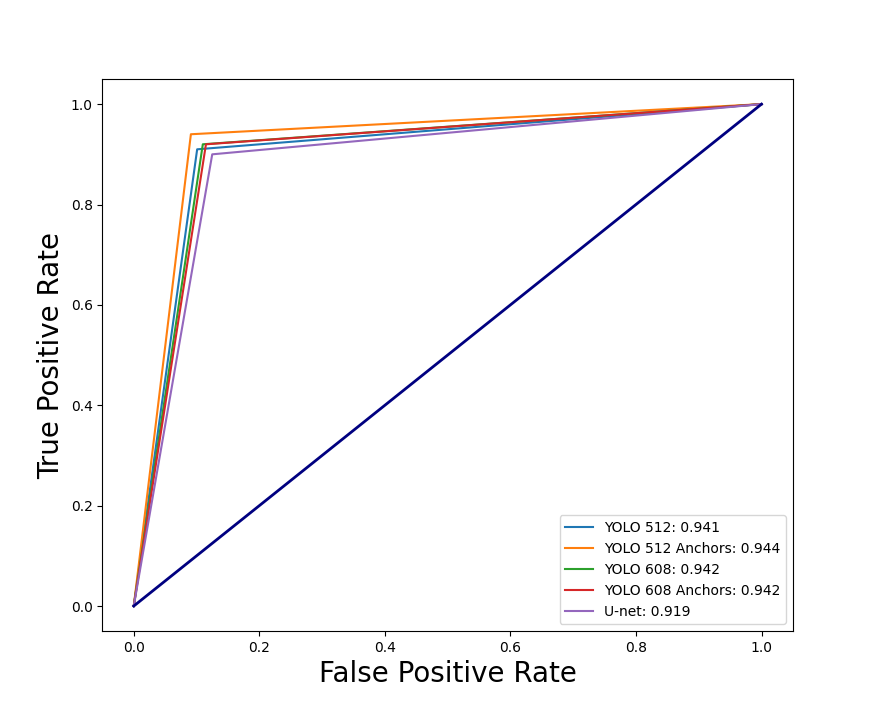
\includegraphics[width=1\textwidth]{images/roc1_new.png}
	\caption{Đường cong ROC cho các đánh giá. Trong phần chú thích của mỗi cấu hình nhỏ bên trong, AUC-ROC được hiển thị cho mọi mô hình - ROC đánh giá nhị phân.}
	\label{fig:roc1}
\end{figure}

\begin{figure}[ht!]
\centering
	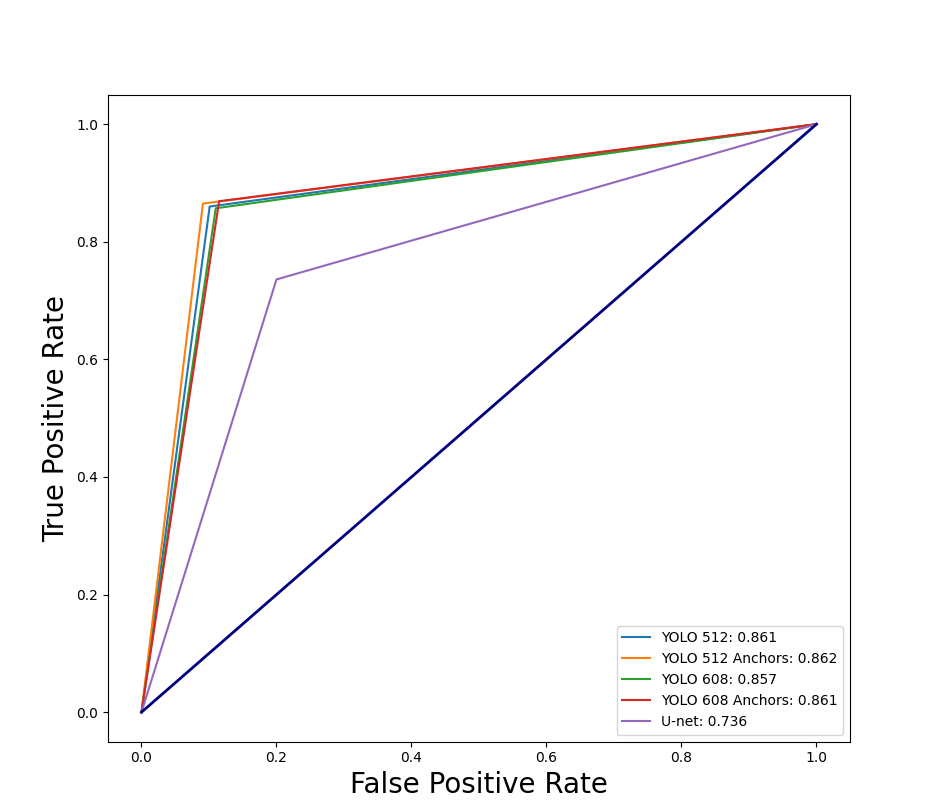
\includegraphics[width=1\textwidth]{images/roc2_new.png}
	\caption{Đường cong ROC cho các đánh giá. Trong phần chú thích của mỗi cấu hình nhỏ bên trong, AUC-ROC được hiển thị cho mọi mô hình - ROC đánh giá dựa trên hình ảnh.}
	\label{fig:roc2}
\end{figure}

\begin{figure}[ht!]
\centering
	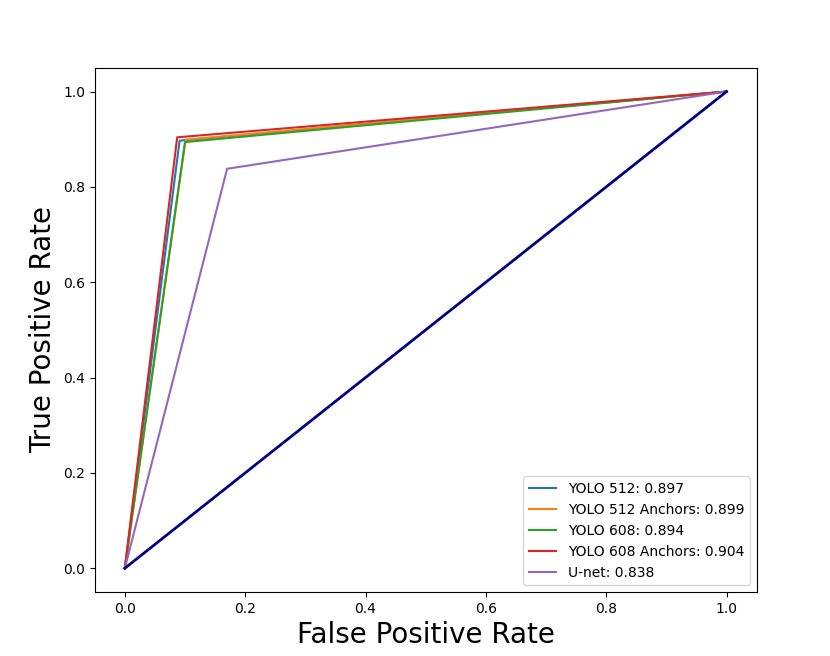
\includegraphics[width=1\textwidth]{images/roc3_new.png}
	\caption{Đường cong ROC cho các đánh giá. Trong phần chú thích của mỗi cấu hình nhỏ bên trong, AUC-ROC được hiển thị cho mọi mô hình - ROC đánh giá dựa trên gãy xương.}
	\label{fig:roc3}
\end{figure}

{\fontsize{13}{12} \selectfont

Hình \ref{fig:roc1} hiển thị các đường cong ROC và giá trị AUC-ROC của mỗi mô hình được thử nghiệm cho đánh giá nhị phân, Hình \ref{fig:roc2} hiển thị các đường cong ROC và giá trị AUC-ROC cho đánh giá dựa trên hình ảnh, và Hình \ref{fig:roc3}  hiển thị các đường cong ROC và giá trị AUC-ROC cho đánh giá dựa trên gãy xương. Kết quả cho thấy mô hình YOLOv4 hoạt động tốt hơn mô hình U-Net. Đối với đánh giá nhị phân, các giá trị ROC-AUC trung bình của các mô hình YOLOv4 là $0,942$, trong khi giá trị AUC-ROC của mô hình U-Net là $0,919$. Kết quả tương tự với đánh giá dựa trên hình ảnh (giá trị AUC-ROC của mô hình YOLOv4 là $0,860$ so với giá trị AUC-ROC của mô hình U-Net là $0,736$), và đánh giá dựa trên gãy xương (mô hình YOLOv4 đạt được giá trị AUC-ROC là $0,899$ trong khi mô hình U-Net đạt được giá trị AUC-ROC là $0,838$).

Để xác nhận thống kê rằng mô hình YOLOv4 hoạt động tốt hơn mô hình U-Net, nghiên cứu đã tiến hành thử nghiệm McNemar. Thử nghiệm cho thấy sự khác biệt đáng kể ở mức $p < 0,05$ giữa tất cả các mô hình dựa trên mô hình YOLOv4 và mô hình U-Net. Tuy nhiên, giữa các mô hình dựa trên YOLOv4, nghiên cứu này nhận thấy không có sự khác biệt đáng kể. Kết quả của thử nghiệm McNemar được mô tả trong các Bảng \ref{tab:mc_binary}.
}


% Bang 1

\begin{table*}[h!]
\centering
\caption{Thử nghiệm McNemar trên kết quả đánh giá nhị phân của các phương pháp. Các giá trị được in đậm thể hiện ý nghĩa thống kê ở mức $p < 0,01$ (in đậm thể hiện giá trị vượt trội).}
\small
\begin{tabular}{|c|c|c|c|c|c|}
\hline
& \multicolumn{1}{|p{2cm}|}{\textbf{YOLO 512}}
& \multicolumn{1}{|p{2cm}|}{\textbf{YOLO 512 \ mỏ neo}}  
& \multicolumn{1}{|p{2cm}|}{\textbf{YOLO 608}}
& \multicolumn{1}{|p{2cm}|}{\textbf{YOLO 608 \ mỏ neo}}
& \multicolumn{1}{|p{2cm}|}{\textbf{U-Net}} 
\\ \hline 
\textbf{YOLO 512}           & 1       & 0,51184   & 0,32108    & 0,23510  &  \textbf{$\bf 2,99 \times 10^{-5}$} \\  \hline
\textbf{YOLO 512 mỏ neo}   & 0,51184       & 1   & 0,08168    & 0,05681   & 
\textbf{$\bf 5,93 \times 10^{-7}$} \\  \hline
\textbf{YOLO 608}           & 0,32108       & 0,08168   & 1    & 0,89568 &    
\textbf{0,00063} \\  \hline
\textbf{YOLO 608 mỏ neo}   & 0,23510       & 0,05681   & 0,89568    & 1 &  
\textbf{0,00167}    \\  \hline
\textbf{U-Net}              & \textbf{$\bf 2,99 \times 10^{-5}$}       & \textbf{$\bf 5,93 \times 10^{-7}$}   & \textbf{0,00063}    & \textbf{0,00167} & 1     \\  \hline

\end{tabular}
\label{tab:mc_binary}
\end{table*}


% Bang 2

% \begin{table*}[h!]
% \centering
% \caption{Thử nghiệm McNemar trên kết quả đánh giá dựa trên hình ảnh của các phương pháp. Các giá trị được in đậm thể hiện ý nghĩa thống kê ở mức $p < 0,01$ (in đậm thể hiện giá trị vượt trội).}
% \small
% \begin{tabular}{|c|c|c|c|c|c|}
% \hline
% & \multicolumn{1}{|p{2cm}|}{\textbf{YOLO 512}}
% & \multicolumn{1}{|p{2cm}|}{\textbf{YOLO 512 \ mỏ neo}}  
% & \multicolumn{1}{|p{2cm}|}{\textbf{YOLO 608}}
% & \multicolumn{1}{|p{2cm}|}{\textbf{YOLO 608 \ mỏ neo}}
% & \multicolumn{1}{|p{2cm}|}{\textbf{U-Net}} 
% \\ \hline 
% \textbf{YOLO 512}           & 1       & 0,48472   & 0,51516    & 0,39979  &  \textbf{$\bf 1.07 \times 10^{-39}$} \\  \hline
% \textbf{YOLO 512 mỏ neo}   & 0,48472       & 1   & 0,16207    & 0,11554  & 
% \textbf{$\bf 1.65 \times 10^{-40}$} \\  \hline
% \textbf{YOLO 608}           & 0,51516       & 0,16207   & 1    & 0,93171  &    
% \textbf{$\bf 6.42 \times 10^{-36}$} \\  \hline
% \textbf{YOLO 608 mỏ neo}   & 0,39979       & 0,11554   & 0,93171    & 1  &  
% \textbf{$\bf 6.40 \times 10^{-37}$}    \\  \hline
% \textbf{U-Net}              & \textbf{$\bf 1.07 \times 10^-39$}       & \textbf{$\bf 1.65 \times 10^{-40}$}   & \textbf{$\bf 6.42 \times 10^{-36}$}    & \textbf{$\bf 6.40 \times 10^{-37}$} & 1     \\  \hline

% \end{tabular}
% \label{tab:mc_image}
% \end{table*}


% Bang 3

% \begin{table*}[h!]
% \centering
% \caption{Thử nghiệm McNemar trên kết quả đánh giá dựa gãy xương của các phương pháp. Các giá trị được in đậm thể hiện ý nghĩa thống kê ở mức $p < 0,01$ (in đậm thể hiện giá trị vượt trội).}
% \small
% \begin{tabular}{|c|c|c|c|c|c|}
% \hline
% & \multicolumn{1}{|p{2cm}|}{\textbf{YOLO 512}}
% & \multicolumn{1}{|p{2cm}|}{\textbf{YOLO 512 \ mỏ neo}}  
% & \multicolumn{1}{|p{2cm}|}{\textbf{YOLO 608}}
% & \multicolumn{1}{|p{2cm}|}{\textbf{YOLO 608 \ mỏ neo}}
% & \multicolumn{1}{|p{2cm}|}{\textbf{U-Net}} 
% \\ \hline 
% \textbf{YOLO 512}           & 1       & 0,14166   & 0,42784    & 0,68905  &  \textbf{$\bf 1.01 \times 10^{-17}$} \\  \hline
% \textbf{YOLO 512 mỏ neo}   & 0,14166       & 1   & 0,02420    & 0,37546  & 
% \textbf{$\bf 2.11 \times 10^{-21}$} \\  \hline
% \textbf{YOLO 608}           & 0,42784       & 0,02420   & 1    & 0,17453  &    
% \textbf{$\bf 8.83 \times 10^{-15}$} \\  \hline
% \textbf{YOLO 608 mỏ neo}   & 0,68905       & 0,37546   & 0,17453    & 1  &  
% \textbf{$\bf 2.72 \times 10^{-19}$}    \\  \hline

% \textbf{U-Net}              & \textbf{$\bf 1.01 \times 10^{-17}$}       & \textbf{$\bf 2.11 \times 10^{-21}$}   & \textbf{$\bf 8.83 \times 10^{-15}$}    & \textbf{$\bf 2.72 \times 10^{-19}$} & 1     \\  \hline

% \end{tabular}
% \label{tab:mc_frac}

% \end{table*}

\subsection{Tóm tắt so sánh các mô hình}

{\fontsize{13}{12} \selectfont
Tóm lại, cả ba tiêu chuẩn đánh giá đều có cùng một kết quả: từ đánh giá nhị phân (có thể được coi là phân loại) không giải thích các quyết định đến phân tích chuyên sâu về sự hiện diện của đứt gãy trong đó mỗi đứt gãy được dự đoán bằng cách sử dụng một hộp giới hạn, các mô hình dựa trên YOLOv4 hoạt động tốt hơn mô hình U-Net. Hơn nữa, chúng ta nhận thấy rằng bản đồ nhiệt đang gặp phải một số vấn đề về hiển thị so với hộp giới hạn. Ví dụ: coi gãy xương như một đối tượng được đại diện bởi hộp giới hạn mang lại kết quả dễ hiểu hơn và thân thiện hơn với con người. Mặc dù không có sự khác biệt đáng kể giữa các mô hình dựa trên YOLOv4 tương ứng, mô hình YOLO 512 mỏ neo luôn đạt được Recall cao nhất, F1 và độ chính xác trong tất cả các thử nghiệm.
}

\section{Vấn đề phát hiện gãy xương và nghiên cứu liên quan}
\label{sec:result_related}

{\fontsize{13}{12} \selectfont
Tổng quan tài liệu về phát hiện gãy xương cổ tay mang lại nhiều cách tiếp cận nghiên cứu thú vị. Để đánh giá và chọn các nghiên cứu quan trọng nhất để so sánh với mô hình dựa trên YOLOv4, nghiên cứu này đã liệt kê các tiêu chí chính được xem xét để số sánh trong Bảng \ref{tab:related}. Các tiêu chí đó như sau:
}

\begin {itemize}
  \item Dữ liệu: số lượng và sự đa dạng dữ liệu được sử dụng trong nghiên cứu.
  \item Mô hình: loại mô hình học máy được sử dụng trong nghiên cứu.
  \item Loại nhận dạng đứt gãy: phân loại, phát hiện hoặc phân đoạn đứt gãy.
  \item Kết quả: báo cáo kết quả về độ chính xác của mô hình.
\end {itemize}

{\fontsize{13}{12} \selectfont
Tiêu chí đầu tiên của nghiên cứu này là xem xét là tập dữ liệu được sử dụng trong nghiên cứu. Mức độ đa dạng ngày càng tăng trong dữ liệu (kim loại, vật đúc, hình chiếu, v.v.) và số lượng dữ liệu khiến mô hình được huấn luyện trên dữ liệu đó trở nên chính xác hơn. Nghiên cứu của Gan \etal \cite{Gan2019}, Thian \etal \cite{Thian2019}, Yahalomi \etal \cite{Yahalomi2019DetectionOD}, và Kim \etal \cite{Kim2018} chỉ tập trung vào một phép chiếu (AP hoặc LAT) và do đó ít phù hợp hơn cho việc ứng dụng vào trong y tế. Olczak \etal \cite{Olczak2017}, Lindsey \etal \cite{Lindsey1806905115}, và Thian \etal \cite{Thian2019} sử dụng hơn 5.000 hình ảnh để huấn luyện mô hình, và đủ để bao gồm tất cả các loại gãy xương khác nhau. Tất cả các nghiên cứu khác sử dụng ít hơn 5.000 hình ảnh, ít đa dạng về các vị trí gãy xương hơn. Về đánh giá mô hình, các nghiên cứu của Bl\"{u}thgen \etal \cite{Blthgen2020}, Yahalomi \etal \cite{Yahalomi2019DetectionOD}, và Kim \etal \cite{Kim2018} sử dụng dưới 300 hình ảnh trong bộ thử nghiệm. Từ nghiên cứu này nhận thấy một số lượng tương đối nhỏ hình ảnh X-quang có thể gây ra sai lệch vì nó không có đủ số lượng trường hợp gãy xương. Cụ thể, trong thực tế, việc phát hiện nhiều vết gãy hoặc theo dõi quá trình chữa lành vết gãy dưới bó bột là những trường hợp không phổ biến nhưng cực kì quan trọng. Các trường hợp này có thể không nằm trong các tập dữ liệu nhỏ, dẫn đến kết quả mô hình rất khó có thể áp dụng vào thực tế. Cuối cùng, sau khi xem xét cẩn thận các mô tả về bộ dữ liệu trong các công trình được đề cập, nghiên cứu này không thể tìm thấy bất kỳ khiếu nại nào liên quan đến việc sử dụng hình ảnh X-quang có chứa kim loại trong đó. Loại hình ảnh X-quang này gây khó khăn hơn trong việc xác định vết gãy, từ đó, mô hình sẽ đạt được hiệu năng tốt hơn khi được huấn luyện trên dữ liệu này.
}

\begin{table*}[h!]
\centering
\caption{Mô tả tổng quan về các nghiên cứu liên quan.}
% \begin{tabularx}{\columnwidth}{|X|X|c|X|X|}
\begin{tabularx}{\columnwidth}{|s|b|s|b|b|}
\hline
\textbf{\#}
& \textbf{Dữ liệu (\# ảnh)}
& \textbf{Mô hình}
& \textbf{Loại\newline nhận dạng}
& \textbf{Kết quả của nghiên cứu}
\\ \hline 

Nghiên cứu này & 
Tổng cộng: 20,327  \newline Huấn luyện: 15.000 \newline Kiểm thử: 1,327 &
YOLOv4 \newline U-Net & Phát hiện gãy xương &
AUC-ROC: 0,899 \newline $F_1$: 0,89997 \newline AUC-ROC: 0,848 \newline $F_1$: 0,83292 \\ \hline


Raisuddin \etal \cite{Raisuddin2021} &
Tổng cộng: 4,497  \newline Huấn luyện: 3,873 \newline Kiểm thử 1: 414  \newline Kiểm thử 2: 210 &
SeresNet50 & Phân loại với phân đoạn bản đồ nhiệt &
AUC-ROC: \#1 0,99 \newline $F_1$: \#1 0,95 \newline AUC-ROC: \#2 0,84 \newline $F_1$: \#2 0,63 \\ \hline


Bl\"{u}thgen \etal \cite{Blthgen2020} &
Tổng cộng: 824  \newline Huấn luyện: 524 \newline Kiểm thử 1: 100  \newline Kiểm thử 2: 200 &
- & Phân loại dựa trên sự chồng chéo bản đồ nhiệt &
AUC-ROC: 0,96, 0,89 \newline $F_1$: 0,95 \\ \hline


Gan \etal \cite{Gan2019} &
Tổng cộng: 2,340  \newline Huấn luyện: 2,040 \newline Kiểm thử: 300 &
Faster R-CNN \& Inception-v4 & Phân loại các vết gãy được phát hiện &
AUC-ROC: 0,96 \newline IoU: 0,87 \\ \hline


Thian \etal \cite{Thian2019} &
Tổng cộng: 14,102  \newline Huấn luyện: 6,515 (AP) / 6,537 (LAT) \newline Kiểm thử: 525 (AP) /  525 (LAT) &
Faster R-CNN  & Phát hiện gãy xương &
AUC ROC: 0,918 (AP) \newline AUC ROC: 0,933 (LAT) \\ \hline


Yahalomi \etal \cite{Yahalomi2019DetectionOD} &
Tổng cộng: 1,432  \newline Huấn luyện: 120 \newline Kiểm thử: 1,312 &
Faster R-CNN  & Phát hiện gãy xương &
ACC: 0,96 \newline MAP: 0,866 \\ \hline


Kim \etal \cite{Kim2018} &
Tổng cộng: 1,489  \newline Huấn luyện: 1,389 \newline Kiểm thử: 100 &
Inception-v3  & Phân loại gãy xương &
AUC ROC: 0,954 \\ \hline


Lindsey \etal \cite{Lindsey1806905115} &
Tổng cộng: 36,390  \newline Huấn luyện: 31,490 \newline Kiểm thử 1: 3,500 \newline Kiểm thử 2: 1,400 &
U-Net  & Phân loại với phân đoạn bản đồ nhiệt &
AUC ROC:  \#1 0,967  \newline AUC ROC: \#2 0,975  \\ \hline


Olczak \etal \cite{Olczak2017} &
Tổng cộng: 256,858  \newline Huấn luyện: 256,458 \newline Kiểm thử 1: 400 &
VGG16  & Phân loại gãy xương &
ACC: 0,83  \\ \hline
\end{tabularx}
\label{tab:related}

\end{table*}

{\fontsize{13}{12} \selectfont
Trên thực tế, bài toán phân loại hình ảnh gãy xương là ít hữu ích nhất đối với các bác sĩ vì nó không cung cấp bất kỳ thông tin chi tiết nào về vị trí có thể bị đứt gãy, cũng như không giải thích được quyết định của mô hình. Olczak \etal \cite{Olczak2017} sử dụng một số cấu trúc liên kết mạng nơ-ron phổ biến (VGG16) để phân loại cổ tay được mô tả trên hình ảnh X-quang là bị gãy một cách chính xác, trong khi Kim \etal \cite{Kim2018} sử dụng mô hìh Inceptionv3 cho cùng một mục đích. Raisuddin \etal \cite{Raisuddin2021} đã thực hiện nhiệm vụ phân loại bằng cách sử dụng mô hình SeresNet50 với phương pháp GradCam để cung cấp giải thích về quyết định của mô hình. Điều này đưa chúng ta đến cái nhìn sâu sắc quan trọng tiếp theo: khả năng giải thích của các vết gãy được phát hiện (mà nhiệm vụ phân loại thiếu). 

Nhiệm vụ phân đoạn là nhiệm vụ chính xác nhất của báo cáo đứt gãy, trong đó mỗi pixel được phân loại là một phần của đứt gãy. Vì vậy, các nghiên cứu của Bl\"{u}thgen \etal \cite{Blthgen2020} và Lindsey \etal \cite{Lindsey1806905115} là những cách phát hiện gãy xương chính xác nhất. Tuy nhiên, các mô hình của họ, DLS và U-net không thành công trong trường hợp cần xác định có nhiều vết gãy trong cùng một khu vực. Cuối cùng, cách tiếp cận mạnh mẽ nhất mà vẫn đảm bảo đủ khả năng giải thích trong khi có thể phân biệt giữa nhiều vết gãy gần đó là phương pháp phát hiện đối tượng. Do đó, Gan \etal \cite{Gan2019}, Thian \etal \cite{Thian2019}, và Yahalomi \etal \cite{Yahalomi2019DetectionOD} tất cả đều sử dụng mô hình Faster R-CNN để phát hiện gãy xương. Mô hình Faster R-CNN là mô hình hai giai đoạn có thể rất khó để tinh chỉnh. Nghiên cứu này muốn chứng minh rằng mô hình một giai đoạn như YOLOv4 (dễ huấn luyện hơn) có thể có được độ chính xác tương đương hoặc thậm chí tốt hơn. Cũng cần phải đề cập rằng các đầu ra mô hình dựa trên phân đoạn (bản đồ nhiệt) có thể dễ dàng chuyển đến các hộp giới hạn bằng cách phân tích nhị phân và ước tính hình chữ nhật giới hạn tối thiểu. Tất cả các nghiên cứu tập trung vào phân khúc và phát hiện gãy xương đều được quan tâm, tuy nhiên, nghiên cứu này nhận thấy rằng phương pháp phát hiện đối tượng có thể có hiệu năng tốt hơn trong trường hợp nhiều vết gãy. 

Hơn nữa, dựa trên kết quả được báo cáo bởi nghiên cứu liên quan và kết quả nghiên cứu, nghiên cứu này không tìm thấy bất kỳ mối liên hệ trực tiếp nào giữa kết quả thu được của các mô hình huấn luyện trước trên một số dữ liệu hoặc khi được huấn luyện bằng cách sử dụng trọng số khởi tạo ngẫu nhiên. Tuy nhiên, đây có thể là một chủ đề cần thiết để nghiên cứu thêm. So sánh về kết quả đạt được, Lindsey\etal \cite{Lindsey1806905115} thu được kết quả tốt nhất. Tuy nhiên, không hoàn toàn công bằng nếu so sánh trực tiếp kết quả của các số liệu cụ thể với nhau. Có thể một mô hình đạt được kết quả tốt hơn trên một tập dữ liệu sẽ hoạt động kém hơn trên tập dữ liệu khác. Để tóm tắt những điều trên, nghiên cứu này kết luận sau:

\begin {itemize}
  \item Đa dạng về dữ liệu: tập dữ liệu phải có các trường hợp mà dữ liệu có các vật thể (kim loại) gây khó khăn cho mô hình hoặc nhiều vết gãy trên các hình chiếu khác nhau. Điều này sẽ làm tăng khả năng khái quát hóa của mô hình được huấn luyện.
 
  \item Cách tiếp cận có sự đánh đổi tốt nhất giữa khả năng giải thích và độ chính xác là cách tiếp cận phát hiện đối tượng. Cụ thể, cách tiếp cận phân đoạn không thành công khi có nhiều vết gãy gần đó.
\end {itemize}
}
\end{document}